\documentclass[12pt]{article}

\usepackage[osf]{libertine}
\usepackage{microtype}
\usepackage[margin=1in]{geometry}
\usepackage{amsmath, amssymb}
\usepackage{pgfplots}
\pgfplotsset{width=10cm,compat=1.15}
\usepackage{tikz}

\title{8th Grade Class Notes}
\author{Ethan Kent}
\date{\today}

\begin{document}

\maketitle

\tableofcontents

\section{Measures of Central Tendency and Spread}

When analyzing a set of data, there are different ways to summarize both the
center of the data and the spread of the data. Two common ways to describe the
center of a dataset are the \emph{median} and the \emph{mean}.

Similarly, two ways to describe how spread out the data are include the
\emph{interquartile range} (IQR) and the \emph{standard deviation}.

Each of these measures has its strengths, particularly when it comes to handling
\emph{outliers}---data points that are significantly higher or lower than the
others.

\subsection{Median and Interquartile Range}

The median is the middle value in a set of data when the numbers are arranged in
order. It splits the data into two equal halves: half of the values are below
the median, and half are above.

The interquartile range (IQR) measures the spread of the middle 50\% of the
data. It is calculated as the difference between the third quartile (the value
below which 75\% of the data falls) and the first quartile (the value below
which 25\% of the data falls).

\begin{figure}[ht]
  \centering
  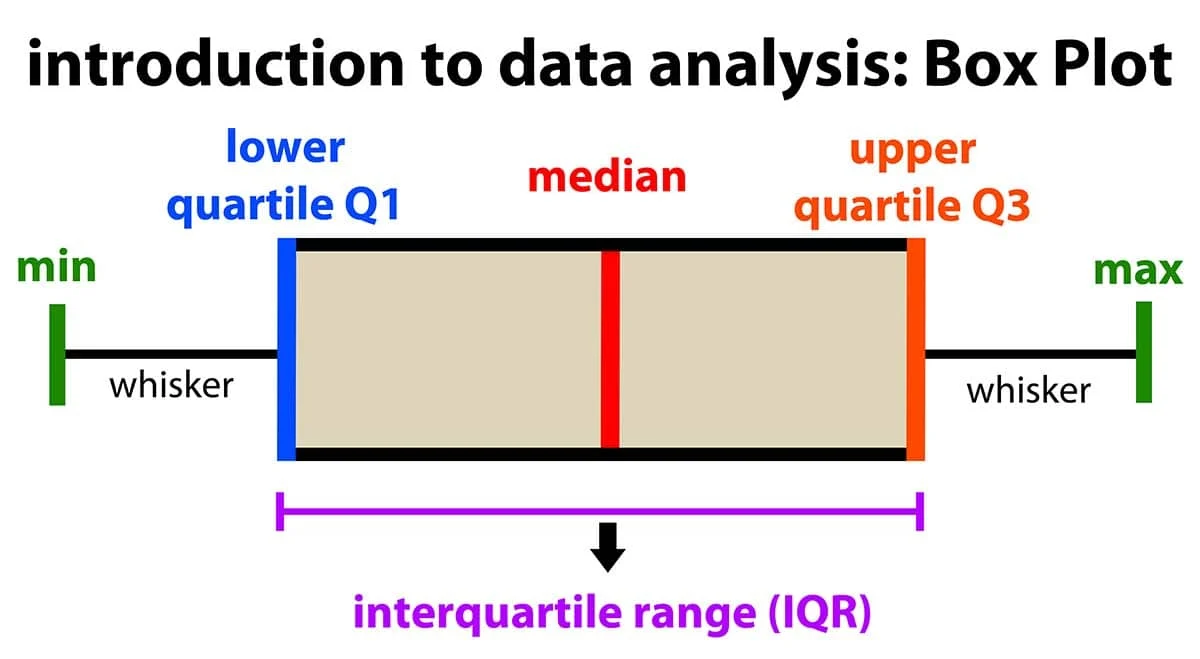
\includegraphics[width=0.5\textwidth]{box-whisker-plot}
  \caption{A box-and-whisker plot showing the distribution of data, highlighting the median, quartiles, and outliers.}
  \label{fig:box-whisker}
\end{figure}

\begin{itemize}
  \item The median and IQR are most useful when the data contains outliers.
        This is because the median is not affected by extremely large or small
        values, while the mean can be pulled significantly in one direction by
        outliers.
  \item For example, consider the incomes of a small group of people. If one
        person in the group is a millionaire, the \emph{mean} income would be
        much higher than most people's actual incomes, making it a misleading
        measure of the ``typical'' income. In this case, the \emph{median}
        income would give a better idea of what most people in the group earn.
\end{itemize}

\textbf{Example:}

\begin{itemize}
  \item Data set: $\{10, 12, 15, 18, 100\}$ (an outlier at 100).
  \item \textbf{Median}: The median is 15, which is a good representation of the
        middle of the data.
  \item \textbf{IQR}: The IQR tells us how spread out the middle 50\% of the
        data is, ignoring the outlier at 100.
\end{itemize}

\subsection{Mean and Standard Deviation}

The mean is the average of the values in a data set. It is found by adding all
the values together and dividing by the number of values. The standard deviation
is a measure of how spread out the numbers are from the mean. A small standard
deviation means that the values are close to the mean, while a large standard
deviation indicates that the values are more spread out.

\begin{itemize}
  \item The mean and standard deviation are best used when the data is
        \emph{symmetric} and does not contain outliers. Because the mean is
        sensitive to extremely large or small values, outliers can skew the
        result and give a misleading picture of the data.
  \item When the data is fairly uniform, the mean provides a good measure of
        central tendency, and the standard deviation gives a clear indication of
        how much the data values vary around the mean.
\end{itemize}

\textbf{Example:}

\begin{itemize}
  \item Data set: $\{10, 12, 15, 18, 20\}$.
  \item \textbf{Mean}: The mean is 15, which accurately reflects the central
        tendency of the data since there are no outliers.
  \item \textbf{Standard Deviation}
        \begin{itemize}
          \item The standard deviation, $\sigma$ (lowercase sigma), gives a
                sense of how closely clustered the data points are around the
                mean. In this population, $\sigma = 3.69$.
          \item If the data set were $\{1, 8, 15, 22, 29\}$, the mean would still
                be 15, but $\sigma = 9.90$
        \end{itemize}


\end{itemize}

\subsection{Choosing Between Median and Mean}

The key difference between using the median or the mean depends on whether your
data contains \emph{outliers}.

\begin{itemize}
  \item If your data has extreme values (outliers), the \emph{median} and
        \emph{IQR} will give you a better understanding of the typical values in
        your data set.
  \item If your data does not have outliers and is relatively symmetric, the
        \emph{mean} and \emph{standard deviation} provide a more precise
        description of both the center and the spread of the data.
\end{itemize}

In summary:
\begin{itemize}
  \item Use the \emph{median} and \emph{IQR} when there are \emph{outliers} or
        a \emph{skewed distribution}.
  \item Use the \emph{mean} and \emph{standard deviation} when the data is
        \emph{symmetrically distributed} and \emph{outlier-free}.
\end{itemize}

\section{Plugging in Numbers for Equations}

You may be asked to solve an equation when given a value for the variable. For
example:

\begin{align*}
  d & = 3l + 2 \quad   & \text{Original equation} \\
  d & = 3(4) + 2 \quad & \text{Substitute } l = 4 \\
  d & = 12 + 2 \quad   & \text{Multiply 3 by 4}   \\
  d & = 14 \quad       & \text{Simplify}
\end{align*}

You might also be asked whether an ordered pair satisfies an equation. To solve
this, remember that an ordered pair represents the $x$ and $y$ values, in that
order. For example, given the equation: $y = 2x - 5$, you can determine if the
ordered pair $(3, 1)$ satisfies the equation by substituting $x = 3$ and $y =
  1$:

\begin{align*}
  y & = 2x - 5         & \text{Original equation}                    \\
  1 & = 2(3) - 5 \quad & \text{Substitute } x = 3 \text{ and } y = 1 \\
  1 & = 6 - 5 \quad    & \text{Multiply 2 by 3}                      \\
  1 & = 1 \quad        & \text{Simplify, the equation is true}
\end{align*}

Since the equation is true when substituting the values, the ordered pair $(3,
  1)$ does satisfy the equation. If the equation were false after substituting the
values, then the ordered pair would not satisfy the equation.

\section{Graphing}

When asked to graph a linear equation on the coordinate plane, there are several
approaches. First, we can make a table by choosing values for $x$ and then
solving for $y$. From this, we can make a table of $x$ and $y$ values, plot
those points on the coordinate plane, and connect the points to form a line.

\subsection{Creating a Table from an Equation}

Let's take the equation \( y = 2x + 1 \). We can create a table by selecting
values for $x$ and calculating the corresponding $y$ values.

\begin{center}
  \begin{tabular}{cc}
    \hline
    $x$  & $y$  \\
    \hline
    $-2$ & $-3$ \\
    $0$  & $1$  \\
    $2$  & $5$  \\
    \hline
  \end{tabular}
\end{center}

Now we can plot the points $(-2, -3)$, $(0, 1)$, and $(2, 5)$ on the coordinate
plane. By connecting these points, we form the line representing the equation \(
y = 2x + 1 \).

\subsection{Graphing Using Point-Slope Form}

You can also take advantage of an equation in point-slope form by remembering
how to find the slope and $y$-intercept. Recall that \emph{slope} is
$\frac{\text{rise}}{\text{run}}$, meaning how much the line goes up (or down)
for every unit it moves horizontally. The slope, denoted as $m$, tells you how
steep the line is, and the $y$-intercept, denoted as $b$, is the point where the
line crosses the $y$-axis.

The general form of a linear equation is:
\[
  y = mx + b
\]
where:
\begin{itemize}
  \item $m$ is the slope (rise/run)
  \item $b$ is the $y$-intercept
\end{itemize}

To graph an equation like \( y = 3x - 2 \), you can start by plotting the
$y$-intercept, which is the point $(0, -2)$. From there, use the slope \( m = 3
\), which means for every 1 unit increase in $x$, $y$ increases by 3 units (rise
of 3 and run of 1). Plot a second point based on this slope, then draw a line
through both points.

\subsection{Graphing Using Slope and $y$-Intercept}

Let's graph the equation \( y = 3x - 2 \). Here's how to do it:

\begin{enumerate}
  \item The $y$-intercept is $-2$, so plot the point $(0, -2)$.
  \item The slope is $3$, which is $\frac{3}{1}$. This means from the
        $y$-intercept, move up 3 units and 1 unit to the right. Plot this second
        point at $(1, 1)$.
  \item Now, connect the two points to form the line.
\end{enumerate}

This is a quick and effective way to graph linear equations without needing to
make a full table of values.

\begin{center}
  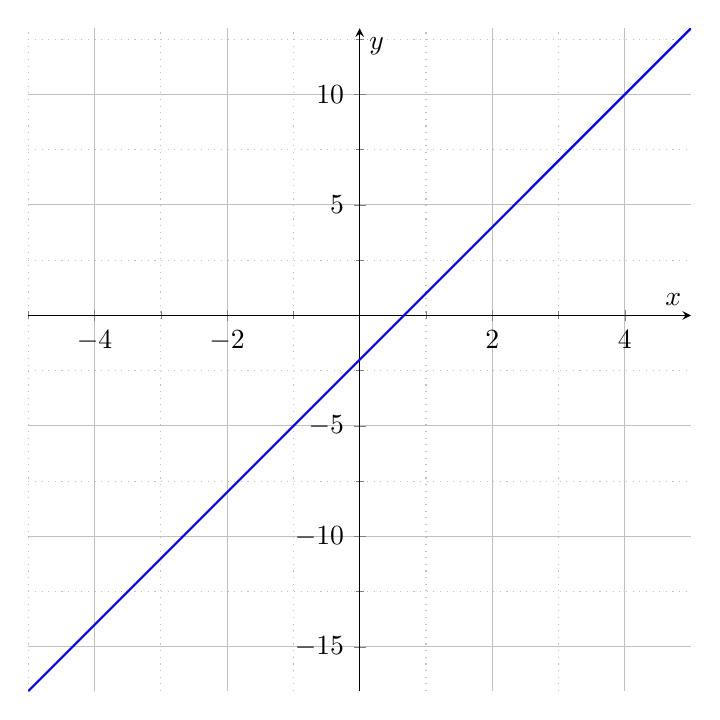
\begin{tikzpicture}
    \begin{axis}[
        axis lines = middle,
        xlabel = {$x$},
        ylabel = {$y$},
        grid = both,
        minor tick num=1,
        major grid style = {lightgray},
        minor grid style = {dotted,lightgray},
        domain=-5:5,
        samples=100,
        width=10cm,
        height=10cm,
      ]
      \addplot[color=blue, thick]{3*x - 2};
    \end{axis}
  \end{tikzpicture}
\end{center}

In this example, the line crosses the $y$-axis at $-2$ and follows a slope of
$3$.

\section{Functions, Function Notation, and Sequences}

A function is similar to the idea of $x$ and $y$ notation, where $x$ represents
an input and $y$ represents the result or output. In basic algebra, you might
have seen equations like

\[
  y = 2x + 3
\]

This is a way of saying that for any value of $x$, we can find $y$ by following
this rule: multiply $x$ by 2, then add 3.

Mathematicians use \emph{function notation} to make this idea more general and
easier to work with. Instead of writing $y = 2x + 3$, we can use function
notation to write

\[
  f(x) = 2x + 3
\]

Here, $f(x)$ is just another way of writing ``the result when you plug $x$ into
the function.'' It’s like a shortcut for showing how $x$ changes into something
else, depending on the rule of the function.

If you want to know what happens when $x = 4$, you would write

\begin{align*}
  f(x) & = 2x + 3 \quad   & \text{Original function}            \\
  f(4) & = 2(4) + 3 \quad & \text{Substitute } 4 \text{ for } x \\
  f(4) & = 8 + 3 \quad    & \text{Multiply } 2 \times 4         \\
  f(4) & = 11 \quad       & \text{Simplify the expression}      \\
\end{align*}

Function notation makes it easier to talk about different rules and to work with
multiple functions at once, which is helpful when solving more complex problems.

A problem set might define several functions and ask you to solve for different
numbers. This can be confusing if they choose different functions just to throw
you off.

A problem set might define several functions and ask you to solve for different
values. This can sometimes be tricky if different functions are used, but it’s
important to focus on the specific rule for each function and apply it
carefully.

Given $f(n) = 8n - 3$ and $g(n) = 3n - 10$, solve $f(1)$, $g(0)$, $f(5)$.

\begin{align*}
  f(1) & = 8(1) - 3 & \text{Multiply } 8 \times 1        \\
  f(1) & = 8 - 3    & \text{Simplify the multiplication} \\
  f(1) & = 5        & \text{Simplify the subtraction}    \\
\end{align*}

\begin{align*}
  g(0) & = 3(0) - 10 & \text{Multiply } 3 \times 0        \\
  g(0) & = 0 - 10    & \text{Simplify the multiplication} \\
  g(0) & = -10       & \text{Simplify the subtraction}    \\
\end{align*}

\begin{align*}
  f(5) & = 8(5) - 3 & \text{Multiply } 8 \times 5        \\
  f(5) & = 40 - 3   & \text{Simplify the multiplication} \\
  f(5) & = 37       & \text{Simplify the subtraction}    \\
\end{align*}

\subsection{Sequences}

You may be given a sequence where you are asked to recognize a pattern, or given
a description of a pattern. A sequence is just an ordered list of numbers, and
often there is a specific rule that determines what comes next. Recognizing the
pattern can help you figure out future numbers in the sequence or fill in
missing terms. It can also be useful to reduce this pattern to an equation,
which allows you to find any term in the sequence without having to write out
the whole list.

For example, consider this situation:

\begin{quote}
  Sarah counted the number of tiles she placed on a wall each day. On the first
  day, she placed 3 tiles. On the second day, she placed 7 tiles. On the third
  day, she placed 11 tiles, and so on. Each day, the number of tiles she placed
  increased by 4 compared to the previous day.
\end{quote}

If we look closely, we can see a pattern: each day Sarah places 4 more tiles
than the previous day. This forms a sequence: 3, 7, 11, 15,~\ldots.

To express this in an equation, we notice that each number in the sequence is
part of a linear pattern. On the first day, she places 3 tiles, on the second
day, she places 7, and on the third day, she places 11. The difference between
each number is 4, so this is an arithmetic sequence.

We can write the rule for the number of tiles Sarah places on day $n$ as:

\[
  a_n = 3 + 4(n - 1)
\]

Here, $a_n$ represents the number of tiles placed on day $n$, and $n$ is the day
number. The number 3 is the starting number (the number of tiles placed on the
first day), and 4 is the amount by which the number of tiles increases each day.
Simplifying the equation:

\[
  a_n = 4n - 1
\]

Now, you can use this equation to find the number of tiles Sarah will place on
any given day without having to continue the sequence manually.

\section{Functions vs. Relations}

\begin{quote}
  A relation is a function if each $x$-value is paired with exactly one
  $y$-value.
\end{quote}

Think of a function as a machine that accepts a number and always spits out the
same result---given that number.

They test this three different ways:

\begin{itemize}
  \item Giving a set of ordered pairs.
  \item Graphing.
  \item Showing a map from Domain to Range.
\end{itemize}

But the concept is the same. Always ask yourself: \emph{Are there any $x$s with
  more than one $y$?}


\subsection{As ordered pairs}

An ordered pair is written in the form $(x, y)$, where $x$ is the input, and $y$
is the output. If no $x$-value is repeated with different $y$-values, then the
relation is a function. For example:

\[
  \{(1,2),(3,4),(5,6),(7,8)\}
\]

This is a function because each $x$-value corresponds to exactly one $y$-value.

However, consider this set:

\[
  \{(2,3),(2,4),(5,6),(7,8)\}
\]

This is not a function because the $x$-value 2 is paired with both 3 and 4,
violating the rule that each $x$-value can only be paired with one $y$-value.

\subsection{As a graph}

Graphing is another way to test if a relation is a function. You can use the
vertical line test: if any vertical line drawn on the graph crosses the relation
more than once, the relation is not a function.

\begin{figure}[h]
  \centering
  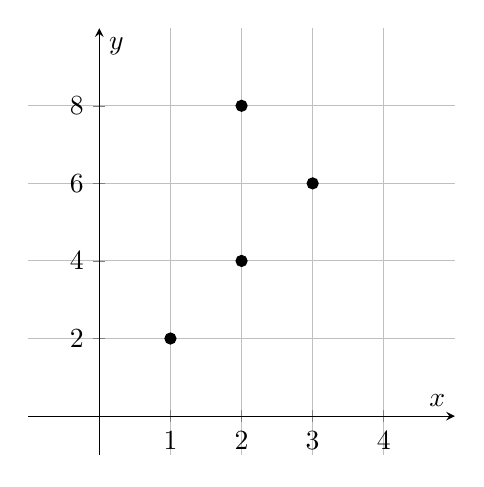
\begin{tikzpicture}
    \begin{axis}[
        axis lines = middle,
        xlabel = $x$,
        ylabel = $y$,
        xmin = -1, xmax = 5,
        ymin = -1, ymax = 10,
        xtick={1, 2, 3, 4},
        ytick={2, 4, 6, 8},
        grid = major,
        width=7cm,
        height=7cm
      ]
      \addplot[only marks, mark=*, mark size=2pt] coordinates {(1, 2) (2, 4) (3, 6) (2, 8)};
    \end{axis}
  \end{tikzpicture}
  \caption{Graph of relation $\{ (1, 2), (2, 4), (3, 6), (2, 8) \}$ fails the vertical line test because $x = 2$ maps to two different $y$-values.}
\end{figure}

\subsection{As a mapping of domain to range}

A function can also be represented by mapping the Domain (the set of all
possible $x$-values) to the Range (the set of all possible $y$-values). For a
relation to be a function, each element in the Domain must map to exactly one
element in the Range.

\begin{figure}[h]
  \centering
  \begin{tikzpicture}[node distance=2cm]
    % Nodes
    \node(D1) at (0, 2) {1};
    \node(D2) at (0, 1) {2};
    \node(D3) at (0, 0) {3};

    \node(R4) at (3, 2) {4};
    \node(R5) at (3, 1) {5};
    \node(R6) at (3, 0) {6};

    % Domain and Range labels
    \node at (-1, 1) {Domain};
    \node at (4, 1) {Range};

    % Arrows
    \draw[->] (D1) -- (R4);
    \draw[->] (D2) -- (R5);
    \draw[->] (D3) -- (R6);
  \end{tikzpicture}
  \caption{Mapping from Domain $\{ 1, 2, 3 \}$ to Range $\{ 4, 5, 6 \}$ shows a function. Each $x$-value in the Domain maps to exactly one $y$-value in the Range.}
\end{figure}

\begin{figure}[h]
  \centering
  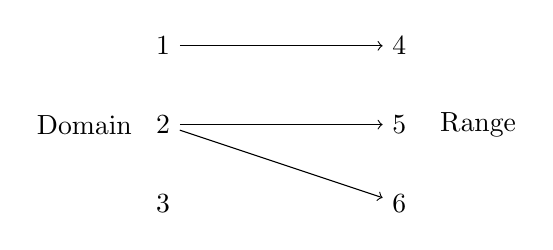
\begin{tikzpicture}[node distance=2cm]
    % Nodes
    \node(D1) at (0, 2) {1};
    \node(D2) at (0, 1) {2};
    \node(D3) at (0, 0) {3};

    \node(R4) at (3, 2) {4};
    \node(R5) at (3, 1) {5};
    \node(R6) at (3, 0) {6};

    % Domain and Range labels
    \node at (-1, 1) {Domain};
    \node at (4, 1) {Range};

    % Arrows
    \draw[->] (D1) -- (R4);
    \draw[->] (D2) -- (R5);
    \draw[->] (D2) -- (R6);
  \end{tikzpicture}
  \caption{Mapping from Domain $\{ 1, 2, 3 \}$ to Range $\{ 4, 5, 6 \}$ is not a function because $2$ in the Domain maps to two different elements in the Range ($5$ and $6$).}
\end{figure}


\end{document}
